\chapter{Current Approaches in Tabular Data Imputation}
\label{chap:ImpReview}

This chapter reviews the imputation methods that form the methodological background for the thesis. Most were developed for general missing-data problems rather than two-phase validation designs. The review first states what each method models and how it generates completed datasets. It then examines the available evidence on coefficient estimation and on the between-imputation variance required for confidence intervals under Rubin's combining rules \citep{Rubin1987}.

A separate set of notation is used in this chapter. Let $\mathcal{D}$ denote the $n \times p$ data matrix, where $\mathcal{D}_{i,j}$ is the realisation of variable $j$ for unit $i$. We treat $\mathcal{D}$ as following a multivariate distribution with unknown parameter vector $\theta$; later sections consider the consequences when this working distribution is misspecified. Let $M$ be an $n \times p$ binary indicator matrix, where $M_{i,j} = 1$ if $\mathcal{D}_{i,j}$ is missing and $M_{i,j} = 0$ otherwise. The partition of $\mathcal{D}$ into observed and missing components is written as $\mathcal{D} = (\mathcal{D}^{\mathrm{obs}}, \mathcal{D}^{\mathrm{mis}})$. These symbols are local to this chapter and differ from the survey sampling notation in Chapters~\ref{chap:SimDesigns}--\ref{chap:SIRD}.


\section{Joint Modelling}
\label{sec:joint}

Joint modelling posits a single multivariate distribution for the complete data, most commonly the multivariate normal, and seeks to characterise the posterior predictive distribution of the missing entries given the observed data:
\begin{equation}
\begin{aligned}
    P(\mathcal{D}^{\mathrm{mis}} \mid \mathcal{D}^{\mathrm{obs}})
    &= \int P(\mathcal{D}^{\mathrm{mis}},\, \theta \mid \mathcal{D}^{\mathrm{obs}}) \, d\theta \\
    &= \int P(\mathcal{D}^{\mathrm{mis}} \mid \mathcal{D}^{\mathrm{obs}},\, \theta)\;
           P(\theta \mid \mathcal{D}^{\mathrm{obs}}) \, d\theta.
\end{aligned}
\label{eq:joint_posterior}
\end{equation}
Except in models with a convenient conjugate or marginal form, drawing from \eqref{eq:joint_posterior} requires the posterior $P(\theta\mid\mathcal{D}^{\mathrm{obs}})$. Its observed-data likelihood can require integration or summation over the missing values. The data augmentation algorithm of \citet{tanner1987calculation} avoids direct evaluation of that observed-data likelihood by alternating between two conditionally tractable steps within a Markov chain Monte Carlo framework. In the imputation step, the missing entries are drawn from $P(\mathcal{D}^{\mathrm{mis}} \mid \mathcal{D}^{\mathrm{obs}},\, \theta^{(t-1)})$ given the current parameter estimate. In the posterior step, a new parameter draw $\theta^{(t)}$ is obtained from $P(\theta \mid \mathcal{D}^{\mathrm{obs}},\, \mathcal{D}^{\mathrm{mis}(t)})$ given the augmented data. Algorithm~\ref{alg:jmda} summarises the procedure.

\begin{algorithm}[t]
\caption{Joint modelling with data augmentation}
\label{alg:jmda}
\begin{algorithmic}[1]
    \Require $\mathcal{D}$: $n \times p$ data matrix; $T$: maximum iterations
    \State Initialise missing entries; obtain $\theta^{(0)}$ from $\mathcal{D}^{(0)}$
    \For{$t = 1, \ldots, T$}
        \State Draw $\mathcal{D}^{\mathrm{mis}(t)} \sim
               P(\mathcal{D}^{\mathrm{mis}} \mid \mathcal{D}^{\mathrm{obs}},\,
               \theta^{(t-1)})$
               \hfill\textit{(imputation step)}
        \State Draw $\theta^{(t)} \sim
               P(\theta \mid \mathcal{D}^{\mathrm{obs}},\,
               \mathcal{D}^{\mathrm{mis}(t)})$
               \hfill\textit{(posterior step)}
    \EndFor
    \State \Return $\mathcal{D}^{\mathrm{mis}(T)}$
\end{algorithmic}
\end{algorithm}

Several \texttt{R} implementations of joint modelling build on \citet{schafer1997analysis}: \texttt{norm} \citep{R-norm} uses a multivariate normal model for continuous data, \texttt{cat} \citep{R-cat} a multinomial log-linear model for categorical data, \texttt{mix} \citep{R-mix} a general location model for mixed data, and \texttt{pan} \citep{R-pan} a multivariate linear mixed model for clustered continuous data. Their dimensional burdens are different. An unstructured covariance matrix in \texttt{norm} has $p(p+1)/2$ free entries. In \texttt{cat}, the number of joint category combinations and possible log-linear interactions can grow much faster as variables and category levels are added. \texttt{mix} combines that categorical model with continuous mean and covariance parameters, while \texttt{pan} estimates fixed effects and unstructured covariance matrices for its multilevel model. These parameter counts can be large relative to the validated sample in our later settings, where the full data dimension can exceed 120.

\citet{honaker2011amelia} proposed an alternative strategy in the package \texttt{Amelia II}, which replaces the MCMC sampler with a bootstrapped expectation-maximisation (EM) algorithm \citep{dempster1977maximum}. Multiple completed datasets are generated by drawing bootstrap replicates of the observed data, fitting the EM algorithm to each replicate, and then imputing from the resulting parameter estimates. This approach reduces computational cost considerably relative to full MCMC, but the validity of the bootstrap approximation to posterior uncertainty depends on the sample size being large relative to the dimension of $\theta$, a condition that may not hold in our high-dimensional two-phase settings where only $5\%$ of the individuals have validated measurements. The multilevel extension \texttt{jomo} \citep{quartagno2015jomo} accommodates hierarchical data structures by allowing covariance matrices to vary across clusters, at the cost of introducing additional parameters that can exacerbate overfitting when the cluster sizes are small.

Joint modelling depends on the assumed joint distribution. Misspecification changes the posterior predictive draws and can then change the downstream analysis \citep{meng1994multiple}. This problem becomes harder to control when the two-phase imputation model covers many error-prone clinical measurements but is fitted to a small validated sample.


\section{Fully Conditional Specification}
\label{sec:fcs}

Fully conditional specification (FCS) circumvents the need to posit a single joint distribution by using a sequence of univariate conditional models \citep{vanBuuren2006, white2011multiple}. Each incomplete variable $\mathcal{D}_j$ is assigned a model $P(\mathcal{D}_j\mid \mathcal{D}_{-j};\theta_j)$, whose parameters are estimated or drawn using the rows on which $\mathcal{D}_j$ is observed. Observed determinants of missingness can be included among the predictors when appropriate; the entire missingness matrix is not automatically part of every conditional model. Multivariate imputation by chained equations (MICE) \citep{van1999multiple} is the most widely used implementation. In each iteration, the algorithm visits each incomplete variable in sequence, draws new parameter values from the corresponding posterior, and then draws its missing entries from the updated conditional distribution. Running the full chain independently $m$ times with different random seeds produces $m$ completed datasets suitable for Rubin's combining rules. Algorithm~\ref{alg:mice} details the procedure.

\begin{algorithm}[t]
\caption{Multivariate imputation by chained equations (MICE)}
\label{alg:mice}
\begin{algorithmic}[1]
    \Require $\mathcal{D}$: $n \times p$ data matrix; $M$: missingness indicator;
             $T$: maximum iterations
    \State Specify $P(\mathcal{D}_j \mid \mathcal{D}_{-j};\theta_j)$ for each incomplete $\mathcal{D}_j$
    \State Initialise missing entries to produce $\mathcal{D}^{(0)}$
    \For{$t = 1, \ldots, T$}
        \State $\mathcal{D}^{(t)} \gets \mathcal{D}^{(t-1)}$
        \For{$j = 1, \ldots, p$ such that $\mathcal{D}_j$ has missing entries}
            \State Form predictor set
                   $\mathcal{D}_{-j}^{(t)} = (\mathcal{D}_1^{(t)}, \ldots, \mathcal{D}_{j-1}^{(t)},\,
                   \mathcal{D}_{j+1}^{(t-1)}, \ldots, \mathcal{D}_p^{(t-1)})$
            \State Draw $\theta_j^{(t)} \sim
                   P(\theta_j \mid \mathcal{D}_j^{\mathrm{obs}},\,
                   \mathcal{D}_{-j}^{(t)})$
            \State Draw $\mathcal{D}_j^{\mathrm{mis}(t)} \sim
                   P(\mathcal{D}_j^{\mathrm{mis}} \mid
                   \mathcal{D}_{-j}^{(t)},\, \theta_j^{(t)})$
            \State Update the missing entries of column $j$
        \EndFor
    \EndFor
    \State \Return $\mathcal{D}^{(T)}$
\end{algorithmic}
\end{algorithm}

The \texttt{mice} package in \texttt{R} \citep{vanBuuren2011} implements this framework. It supports correlation-based predictor screening (\texttt{quickpred}), conditional models for continuous, binary, ordinal and nominal variables, and predictive mean matching \citep{little1988missing}. Predictive mean matching draws from observed donors rather than a parametric predictive distribution. The imputations therefore stay within the observed support, and their sensitivity to a misspecified conditional mean model can be lower than for direct parametric draws \citep{morris2014tuning}. The separate conditional specifications can also include non-linear transformations and interaction terms \citep{vanBuuren2018}.

The flexibility of FCS comes at a theoretical cost. Because the conditional models are specified separately, there is no guarantee that they are mutually compatible, that is, that a joint distribution consistent with all of the specified conditionals exists \citep{vanBuuren2018, white2011multiple}. An incompatible chain may still converge to a stationary distribution, but that distribution need not have the specified models as its full conditionals and can depend on the order in which variables are updated. The joint-model interpretation and the corresponding inferential guarantees are then unclear. This matters more as the number of conditional models grows and each must be estimated from the observed entries of its target variable. For dense regression conditionals, the principal matrix calculations can scale as roughly $O(np^2+p^3)$ per chained-equation iteration, and more iterations may be required in higher dimensions. Overfitting becomes a further concern when the number of predictors approaches or exceeds the number of observed entries in the target column \citep{zhu2015multiple, deng2016multiple}.

\section{Tree-Based and Ensemble Methods}
\label{sec:trees}

Decision trees provide a non-parametric framework for conditional modelling by partitioning the covariate space recursively into disjoint regions, within each of which the response is approximated by a constant \citep{breiman1984classification}. At each node, the algorithm identifies the variable and split point that minimise a cost function, such as the sum of squared errors for continuous responses or the Gini impurity index for categorical responses. This recursive structure captures non-linear relationships and high-order interactions without requiring their explicit specification, a property that is attractive for imputation models where the functional form linking the phase-one auxiliaries to the phase-two targets is typically unknown.

\citet{burgette2010multiple} integrated classification and regression trees into the MICE framework for multiple imputation. Their approach drew imputed values from the terminal node distributions using a Bayesian bootstrap, but the tree structure itself was held fixed across the $m$ completed datasets. This design choice constrained the between-imputation variance to reflect only the sampling variability within the terminal nodes, not the structural uncertainty in the tree topology. The resulting confidence intervals were systematically too narrow. \citet{doove2014recursive} addressed this limitation by fitting trees to bootstrapped versions of the observed data, so that the tree structure varied across imputations. Their implementation is available in \texttt{mice} as \texttt{mice.impute.cart} for single trees and \texttt{mice.impute.rf} for random forests.

A single deep tree is prone to overfitting; a single shallow tree underfits. Ensemble methods address this tension by averaging many trees. Random forests \citep{breiman2001random} train the trees on bootstrap samples and consider a random subset of candidate variables at each split. \citet{stekhoven2012missforest} proposed \texttt{missForest}, which iterates between imputing each variable and refitting its forest until convergence. Forest averaging yields point predictions that approximate $\mathrm{E}(\mathcal{D}_j^{\mathrm{mis}} \mid \mathcal{D}_{-j})$ rather than draws from the full conditional distribution. The method returns one completed dataset, so it supplies no between-imputation variance and cannot by itself be analysed with Rubin's multiple-imputation rules. Repeating the same point-prediction procedure would not represent the missing conditional spread. \citet{mayer2019package} reimplemented \texttt{missForest} using the faster \texttt{ranger} backend \citep{wright2017ranger}, but the single-imputation limitation persists. The random forest variant within \texttt{mice} (\texttt{mice.impute.rf}), proposed by \citet{doove2014recursive}, instead draws imputed values from the empirical distribution in the terminal node to which each missing case is assigned. Repeating the MICE procedure $m$ times generates between-imputation variation, although finite-sample calibration is not guaranteed.

Boosting methods build trees sequentially rather than in parallel. The original AdaBoost algorithm \citep{freund1997decision} achieves this by reweighting the training observations at each iteration, assigning higher weight to cases that were misclassified by the previous tree. Gradient boosting \citep{friedman2001greedy} generalises this idea by fitting each successive tree to the pseudo-residuals of the current ensemble, so the algorithm performs a form of functional gradient descent that primarily targets bias reduction. XGBoost \citep{chen2016xgboost} extends the gradient boosting framework with a regularised objective function that penalises tree complexity and exploits second-order curvature information for more accurate split selection. A distinctive feature of XGBoost for missing data applications is that it learns optimal default splitting directions for missing predictor values during tree construction, so no separate imputation pass over the predictors is required at each iteration of the chained equations.

\citet{deng2024multiple} developed \texttt{mixgb}, an XGBoost-based multiple imputation method for tabular data. The original publication and the current package use different defaults. In the current implementation, stochastic variation across the $m$ completed datasets comes from the row subsampling used within XGBoost, without an additional bootstrap \citep{deng2026mixgb}. Predictive mean matching remains available as an option, but the current default is \texttt{pmm.type = NULL}; the thesis uses this default and therefore does not apply predictive mean matching. Algorithm~\ref{alg:mixgb} describes that implementation.

\begin{algorithm}[t]
\caption{Multiple imputation through XGBoost (MIXGB)}
\label{alg:mixgb}
\begin{algorithmic}[1]
    \Require $\mathcal{D}$: $n \times p$ data matrix; $M$: missingness indicator;
             $T$: maximum iterations; $m$: number of completed datasets;
             optional \texttt{pmm.type}
    \For{$d = 1, \ldots, m$}
        \State Initialise the missing entries to produce $\mathcal{D}^{(d,0)}$
        \For{$t = 1, \ldots, T$}
            \State $\mathcal{D}^{(d,t)} \gets \mathcal{D}^{(d,t-1)}$
            \For{$j = 1, \ldots, p$ such that $\mathcal{D}_j$ has missing entries}
                \State Fit XGBoost for $\mathcal{D}_j$ using its observed rows and the
                       configured internal row and column subsampling
                \State Predict the missing entries of $\mathcal{D}_j$
                \If{\texttt{pmm.type} is not \texttt{NULL}}
                    \State Replace the predictions by the selected donor matches
                \EndIf
                \State Update the missing entries of column $j$
            \EndFor
        \EndFor
    \EndFor
    \State \Return $\mathcal{D}^{(1,T)},\ldots,\mathcal{D}^{(m,T)}$
\end{algorithmic}
\end{algorithm}

The XGBoost model in \texttt{mixgb} has several interacting hyperparameters, including the learning rate, tree depth, row and column subsampling fractions, and regularisation penalties \citep{chen2016xgboost}. In the two-phase settings studied here, the phase-two targets may be observed for only $5\%$ of the cohort, so these choices are estimated from a much smaller sample than the cohort size suggests. Section~\ref{sec:tuning} therefore tunes \texttt{mixgb} within each setting.


\section{Deep Generative Models}
\label{sec:deep_gen}

Joint modelling already treats the incomplete variables through one multivariate distribution. FCS and the chained tree and boosting methods instead construct conditional models one variable at a time. Deep generative methods use neural networks to represent flexible joint or conditional distributions, although the precise object depends on the architecture and training objective. This section reviews autoencoders and their variational extensions, generative adversarial networks, and diffusion models.


\subsection{Autoencoders and Variational Inference}
\label{sec:ae_vae}

An autoencoder consists of an encoder $f_{\phi}$ that maps the input $x \in \mathbb{R}^p$ to a latent representation $h = f_{\phi}(x) \in \mathbb{R}^d$ with $d < p$, and a decoder $g_{\psi}$ that reconstructs the input as $\hat{x} = g_{\psi}(h)$. The pair $(f_{\phi}, g_{\psi})$ is trained jointly to minimise a reconstruction loss, typically the mean squared error. An undercomplete bottleneck limits the information passed to the decoder and can encourage a compressed representation of structure shared across variables, though compression alone gives no guarantee of noise removal. Nonlinear autoencoders are often motivated by the manifold hypothesis, under which high-dimensional data concentrate near a lower-dimensional submanifold \citep{bengio2013representation, goodfellow2016deep}.

The denoising autoencoder (DAE) trains a network to reconstruct clean data $x$ from deliberately corrupted inputs $\tilde{x}$ \citep{vincent2008extracting}. The corruption can use additive Gaussian noise, random masking, or both. Predicting the removed values requires the network to use dependencies available in the uncorrupted inputs, although the objective does not guarantee that every relevant dependency is retained. For small Gaussian corruption, \citet{alain2014regularized} relate the optimal local reconstruction displacement to the score of the data density. The separate principal-component result applies to an undercomplete linear autoencoder with quadratic reconstruction loss \citep{baldi1989neural}. Under squared reconstruction loss, the optimal point prediction is the conditional mean of the clean value given the corrupted input. A DAE can provide an imputation function, but its reconstruction objective alone does not generate draws from the full conditional distribution.

\citet{gondara2018mida} proposed multiple imputation using denoising autoencoders (MIDA). It uses an overcomplete architecture in which the hidden dimension $d$ exceeds the input dimension $p$. The method trains the network $m$ times from different random initialisations to produce $m$ completed datasets. This is computationally expensive, and the variation across the fitted networks is not guaranteed to equal the required between-imputation variance. \citet{lall2022midas} proposed multiple imputation with denoising autoencoders (MIDAS), which trains one DAE and uses Monte Carlo dropout \citep{gal2016dropout} to vary its predictions across completed datasets. The interpretation of dropout as an approximate deep Gaussian process \citep{damianou2013deep,gal2016dropout} does not determine whether the resulting between-imputation variance is calibrated; that also depends on the dropout rate and the fitted network.

A standard DAE returns one reconstruction for a fixed input. Repeated training and Monte Carlo dropout add variation across completed datasets, but the reconstruction objective itself does not specify a conditional sampling distribution. A variational autoencoder (VAE) \citep{kingma2013auto} instead introduces a probabilistic latent variable $u$ and models the joint distribution $p(x, u) = p(x \mid u)\, p(u)$. The encoder outputs the parameters $(\mu_{\phi}, \sigma_{\phi})$ of an approximate posterior $q_{\phi}(u \mid x)$, and the latent variable is sampled via the reparameterisation $u = \mu_{\phi} + \sigma_{\phi} \odot z$ with $z \sim \mathcal{N}(0, I)$ \citep{rezende2014stochastic}. Training maximises the evidence lower bound (ELBO),
\begin{equation}
    \mathcal{L}(\phi, \psi)
    = \mathrm{E}_{q_{\phi}(u \mid x)}
      \bigl[\log p_{\psi}(x \mid u)\bigr]
    - D_{\mathrm{KL}}\bigl(q_{\phi}(u \mid x) \;\|\; p(u)\bigr),
    \label{eq:elbo}
\end{equation}
where the first term is the expected reconstruction likelihood and the second is the Kullback--Leibler (KL) divergence \citep{kullback1951information} between the approximate posterior and the prior. The ELBO balances reconstruction accuracy against regularisation of the latent space. Different draws of $u$ can then be decoded to produce multiple imputations.

Several VAE-based imputation methods have been proposed, differing primarily in how they handle partial observation and how they generate the $m$ completed datasets. \citet{nazabal2020handling} introduced the Heterogeneous-Incomplete VAE (HI-VAE), which accommodates mixed variable types by specifying tailored likelihood functions in the decoder for continuous, categorical, and ordinal variables, and marginalises over the missing entries in the ELBO. \citet{ivanov2018variational} proposed the variational autoencoder with arbitrary conditioning (VAEAC), which conditions the encoder and decoder on the set of observed features directly, allowing the model to handle arbitrary patterns of missingness in a single forward pass. They found that performance degrades when the training and test missingness-pattern distributions differ. For two-phase use, the relevant question is therefore whether the artificial training masks represent the phase-two application pattern.

\citet{mattei2019miwae} developed the missing-data importance-weighted autoencoder (MIWAE), which tightens the ELBO bound by using importance-weighted estimates of the observed-data log-likelihood. Multiple imputations are generated by drawing $L$ latent variables from the approximate posterior for each observation, decoding each into a completed data vector, and selecting $m$ candidates through sampling importance resampling. \citet{ma2023mivae} introduced multiple imputation based on a variational autoencoder (MIVAE), which adds a corrupted input layer that simulates missingness patterns during training.

\citet{deng2024thesis} developed \texttt{miae}, an autoencoder imputation package with a denoising-autoencoder variant that uses Monte Carlo dropout (\texttt{midae}) and a variational-autoencoder variant (\texttt{mivae}). In contrast to most autoencoder imputation studies, which report only reconstruction accuracy, that work assessed the downstream inference. Its coefficient results were comparable to those from the tree-based methods in \texttt{mice}, but the imputation variability was not represented adequately; in particular, \texttt{mivae} under-stated the between-imputation variance. Reflecting that variability correctly was identified as the main obstacle to valid multiple imputation with autoencoders.

The VAE approximation can affect the conditional distribution used for imputation. The ELBO may be loose when $q_{\phi}(u\mid x)$ is restricted to a factorised Gaussian, and KL regularisation can suppress features of the conditional distribution that are weakly represented in the latent space \citep{mattei2019miwae}. These are possible sources of error for VAE imputations, not established explanations for coefficient bias or interval coverage. No VAE is evaluated in this thesis, so the results for SICG and SIRD cannot be attributed to these VAE-specific mechanisms. Section~\ref{sec:uncertainty_gap} treats separately the fitted-model uncertainty that can be omitted by any generative method used in a single-fit pipeline.


\subsection{Generative Adversarial Networks}
\label{sec:gans}

Generative adversarial networks (GANs) \citep{goodfellow2014generative} replace the likelihood-based training objective with an adversarial game between a generator $G$ and a discriminator $D$. The generator maps a latent noise vector $z \sim p_z(z)$ to the data space, and the discriminator is trained to distinguish between samples drawn from the empirical data distribution $p_{\mathrm{data}}$ and samples produced by $G$. The two networks are optimised jointly through the minimax objective
\begin{equation}
    \min_G \max_D \; V(D, G)
    = \mathrm{E}_{x \sim p_{\mathrm{data}}}[\log D(x)]
    + \mathrm{E}_{z \sim p_z}[\log(1 - D(G(z)))].
    \label{eq:gan_obj}
\end{equation}
\citet{goodfellow2014generative} showed that, under an optimal discriminator, the generator minimises the Jensen--Shannon divergence between $p_{\mathrm{data}}$ and the model distribution $p_g$ \citep{lin1991divergence}. In finite training, the generator and discriminator need not reach that optimum. Because the discriminator supplies the training signal through data-dependent gradients rather than through a global likelihood, the generator is pushed to produce samples that are realistic along the directions the discriminator uses to separate real from generated records. This mechanism yields sharp samples but invites a characteristic failure, mode collapse, in which the generator concentrates its output on a limited set of regions and fails to represent other parts of the distribution.

In the context of missing data, \citet{yoon2018gain} proposed Generative Adversarial Imputation Nets (GAIN), the first GAN-based imputation framework. The generator receives the partially observed data vector $\tilde{x}$, with missing entries replaced by noise, together with the missingness mask, and returns completed values. The discriminator predicts the observed-or-imputed status of each component. A hint matrix reveals part of the true mask while leaving other components for the discriminator to infer; this partial information is used in the original identification argument. The generator loss combines the adversarial signal with a reconstruction penalty on the observed entries. In the original formulation this penalty is weighted by a single hyperparameter $\alpha$; following the adaptation of GAIN to a clinical dataset by \citet{dong2021gain}, the implementation used here applies $\alpha$ to continuous variables and a separate weight $\beta$ to categorical variables encoded via one-hot representation.

The hint does not change a vector-level discriminator into a componentwise one; the discriminator is componentwise throughout. Its role is to provide enough mask information for the desired conditional distribution to be identified \citep{yoon2018gain}. The hint rate and the reconstruction weights are therefore tuning parameters in the thesis implementation. A large squared-error reconstruction contribution can favour values near the conditional mean and reduce imputation spread. That mechanism does not by itself establish memorisation or adversarial mode collapse, which require separate evidence.

Subsequent work has proposed various architectural modifications to GAIN. \citet{wang2021pc} incorporated pseudo-label conditioning (PC-GAIN), \citet{friedjungova2020missing} used a Wasserstein generative adversarial imputation network (WGAIN), and \citet{neves2021sgain} added a gradient penalty to its Wasserstein variant (WSGAIN-GP). These variants address specific training stability issues but were designed primarily for single imputation. The multiple-imputation extension of \citet{dai2021multiple} fits a conditional GAN for each blockwise missingness pattern. Its MI-GAN$_1$ procedure trains from complete cases, whereas MI-GAN$_2$ iterates over the full incomplete dataset after an initial imputation. To obtain multiple completed datasets, the training algorithm is rerun, so fitted-network variation and the pattern-specific fits are two separate parts of the procedure.

For coefficient estimation, a GAN must recover the features of the conditional distribution on which the analysis depends. Figure~\ref{fig:gain_underdispersion} illustrates one failure under Simulation Design~II. Only the exposure is imputed; for the unvalidated units the imputed exposure is concentrated near its conditional mean given the outcome, so its spread is compressed and the fitted exposure--outcome line steepens away from the truth. Because the imputed exposure still tracks the outcome, this is under-dispersion of the conditional draw rather than a collapse of the exposure distribution, and it is consistent with the squared-error reconstruction term favouring values near the conditional mean noted above.

\begin{figure}[htbp]
\centering
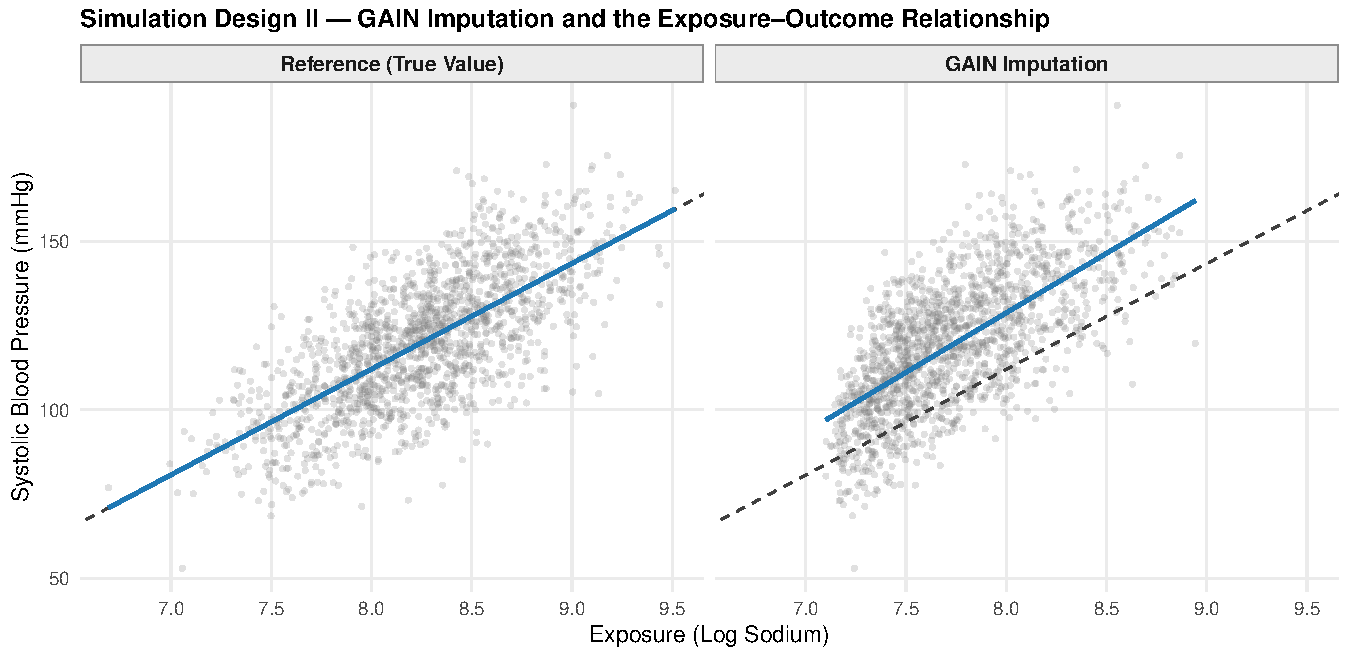
\includegraphics[width=\textwidth]{gain_underdispersion.pdf}
\caption{A trained GAIN model under Simulation Design~II, on a single replicate under simple random sampling. Each panel plots the Gaussian outcome against the exposure for the unvalidated units: the left panel uses the true exposure and the right the GAIN imputation. The dashed line is the true regression fit, repeated in both panels, and the solid line is the fit within each panel. In the right panel the imputed exposure is concentrated near its conditional mean given the outcome, so its spread is compressed and the fitted exposure--outcome line steepens, which is the mechanism by which the distorted imputation biases the downstream coefficient $\hat{\beta}$.}
\label{fig:gain_underdispersion}
\end{figure}


\subsection{Diffusion Models}
\label{sec:diffusion}

Score-based diffusion models \citep{sohl-dickstein2015deep, song2020score} define a forward Markov chain that progressively corrupts a data sample $x_0 \sim q(x)$ into pure noise by adding Gaussian perturbations over a sequence of time steps $t = 1, \ldots, T$. Under the denoising diffusion probabilistic model (DDPM) framework of \citet{ho2020denoising}, the forward transitions are
\begin{equation}
    q(x_t \mid x_{t-1})
    = \mathcal{N}\bigl(x_t;\; \sqrt{1 - \beta_t}\, x_{t-1},\;
      \beta_t I\bigr),
    \label{eq:ddpm_forward}
\end{equation}
where $\{\beta_t\}_{t=1}^T$ is a variance schedule chosen so that $x_T$ is approximately distributed as $\mathcal{N}(0, I)$ for sufficiently large $T$. The generative model parameterises the reverse transitions $p_{\theta}(x_{t-1} \mid x_t)$ and is trained by minimising a reweighted variational bound on the negative log-likelihood, which reduces to a sequence of denoising objectives \citep{ho2020denoising}. The simplified loss function is
\begin{equation}
    L_{\mathrm{DM}}
    = \mathrm{E}_{x_0,\, z \sim \mathcal{N}(0,I),\, t}
    \bigl[\lVert z - z_{\theta}(\sqrt{\bar{\alpha}_t}\, x_0
    + \sqrt{1 - \bar{\alpha}_t}\, z,\; t) \rVert^2\bigr],
    \label{eq:ddpm_loss}
\end{equation}
where $\bar{\alpha}_t = \prod_{s=1}^{t}(1 - \beta_s)$ and $z_{\theta}$ is the noise prediction network.

The connection to score-based modelling \citep{song2019generative, song2020score} provides an alternative perspective: the network learns the score function $\nabla_x \log p_t(x)$, the gradient of the log of $p_t$, where $p_t$ denotes the marginal density after $t$ forward-noising steps, and generation proceeds along the learned score field. Diffusion training does not use the adversarial objective that gives rise to GAN mode-collapse dynamics. A fitted finite network can still approximate the score poorly or miss parts of the target distribution, so the construction does not guarantee complete mode coverage.

For imputation, the reverse diffusion process is conditioned on the observed entries. The conditional score function $\nabla_{x^{\mathrm{mis}}} \log p_t(x^{\mathrm{mis}} \mid x^{\mathrm{obs}})$ guides denoising of the missing entries. \citet{tashiro2021csdi} introduced the Conditional Score-based Diffusion model for Imputation (CSDI), using separate attention modules for temporal and feature dependencies. \citet{zheng2022diffusion} adapted it to tabular data as TabCSDI by removing temporal attention and representing categorical variables through one-hot encoding, analog bits, or feature tokenisation. These representations allow the score model to process mixed data in an encoded continuous space. They do not give TabCSDI a separate multinomial diffusion kernel; that distinction becomes relevant for SIRD in Chapter~\ref{chap:SIRD}.

Several recent extensions have addressed specific limitations of the original diffusion imputation framework. \citet{zhang2025diffputer} combined the EM algorithm with score-based models to handle training on incomplete data, iteratively refining the joint distribution estimate. \citet{liu2024simpdm} introduced self-supervised alignment to reduce sensitivity to the initial noise realisation. \citet{villaizan2025mtabgen} proposed an encoder-decoder transformer with multinomial and Gaussian diffusion kernels to handle heterogeneous feature types in a unified architecture. \citet{zhou2025missddim} adopted non-Markovian deterministic sampling paths to accelerate inference, reducing the number of reverse steps required without sacrificing imputation quality.

Repeated reverse-diffusion runs from different initial noise values provide stochastic draws from the fitted conditional distribution, so one trained model can generate multiple completed datasets. These runs represent variation conditional on the fitted network. They do not vary its fitted parameters and therefore do not constitute the posterior step required for proper multiple imputation. The simulations examine separately whether the resulting coefficient estimates are centred and whether the reported intervals cover under two-phase sampling.

\section{Applicability to Two-Phase Designs}
\label{sec:two_phase_applicability}

The remaining question is which methods have been evaluated for coefficient and interval estimation in settings comparable to a two-phase validation design.

\subsection{Divergent Evaluation Standards in Statistics and Computer Science}
\label{sec:3.5.1}

The statistical and machine-learning literatures have usually evaluated imputation for different purposes. In statistics, imputation is used to support estimation and uncertainty quantification for an analysis parameter $\beta$ \citep{Rubin1987, meng1994multiple}. Relevant evaluations therefore examine the downstream estimator, including its bias and confidence-interval coverage. Section~\ref{sec:eval_metrics} adds oracle diagnostics that separate displacement of the estimate from miscalibration of its standard error. Pointwise prediction error does not answer either question.

In the computer science and machine learning literature, imputation is more commonly treated as a prediction or distribution-recovery task. The most commonly reported evaluation metrics are the root mean squared error (RMSE) between imputed and held-out true values, the mean absolute error (MAE), and, in more recent work, distributional distances such as the Wasserstein distance or maximum mean discrepancy (MMD). Some studies also report predictive performance from a classifier trained on the completed data, using measures such as the area under the receiver operating characteristic curve (AUROC) or the F1 score. These metrics do not, by themselves, establish the bias or interval coverage of a regression estimator fitted to the completed data.

\citet{naf2023imputation} showed across fifteen real datasets that RMSE can favour conditional-mean predictors over methods that draw from a conditional distribution. \citet{naf2025mar} formulated imputation as distributional prediction and advocated proper scoring rules rather than pointwise error alone. These results explain why pointwise and distributional evaluations can rank methods differently. They do not replace direct evaluation of coefficient bias or interval coverage.

\subsection{Evaluation Practices in the Existing Literature}
\label{sec:3.5.2}
To make this divergence concrete, Table~\ref{tab:eval_metrics_lit} catalogues the evaluation metrics reported in the original papers for each imputation method discussed in this chapter. The metrics are classified into three categories: \emph{data-level} metrics that measure pointwise prediction accuracy (RMSE, MAE, classification accuracy); \emph{distribution-level} metrics that assess whether the imputed data recover the joint or marginal distribution of the original data (Wasserstein distance, MMD, energy distance, KL divergence, distributional plots); and \emph{inference-level} metrics that evaluate the properties of a downstream statistical estimator fitted to the imputed data (bias of $\hat{\beta}$, confidence interval coverage, SE ratio, type~I error rate). A method is marked as reporting a given metric only if the original paper includes it in the primary evaluation; downstream prediction accuracy (e.g., AUROC of a classifier) is classified under data-level because it measures predictive performance rather than inferential validity.

\begin{table}[ht]
\centering
\caption{Evaluation metrics reported in the original publications of the imputation methods reviewed in this chapter. A tick (\checkmark) indicates the metric was reported; a dash (--) indicates it was not. Column headers: \textbf{D} = data-level (pointwise prediction); \textbf{Dist} = distribution-level (distributional agreement); \textbf{Inf} = inference-level (downstream statistical inference). For the statistical methods in the first two groups, inference-level evaluation refers to the demonstration of valid inference via Rubin's combining rules, which may take the form of a formal simulation study or an applied analysis reporting bias, variance components, and confidence intervals.}
\label{tab:eval_metrics_lit}
\small
\setlength{\tabcolsep}{4pt}
\begin{tabularx}{\textwidth}{>{\raggedright\arraybackslash}Xccc}
\hline
\textbf{Method} & \textbf{D} & \textbf{Dist} & \textbf{Inf} \\
\hline
\multicolumn{4}{l}{\textit{Joint modelling and FCS}} \\
\texttt{norm/cat/mix} \citep{schafer1997analysis} & -- & -- & \checkmark \\
\texttt{Amelia II} \citep{honaker2011amelia} & -- & -- & \checkmark \\
\texttt{mice} (PMM) \citep{vanBuuren2011} & -- & -- & \checkmark \\
\texttt{jomo} \citep{quartagno2015jomo} & -- & -- & \checkmark \\[2pt]
\multicolumn{4}{l}{\textit{Tree-based and ensemble methods}} \\
\texttt{mice.impute.cart/.rf}$^{\dag}$ \citep{burgette2010multiple, doove2014recursive} & -- & -- & \checkmark \\
\texttt{missForest} \citep{stekhoven2012missforest} & \checkmark & -- & -- \\
\texttt{mixgb} \citep{deng2024multiple} & -- & -- & \checkmark \\[2pt]
\multicolumn{4}{l}{\textit{Autoencoders and VAEs}} \\
MIDA \citep{gondara2018mida} & \checkmark & -- & -- \\
MIDAS \citep{lall2022midas} & \checkmark & -- & \checkmark \\
HI-VAE \citep{nazabal2020handling} & \checkmark & -- & -- \\
VAEAC \citep{ivanov2018variational} & \checkmark & -- & -- \\
MIWAE \citep{mattei2019miwae} & \checkmark & -- & -- \\
MIVAE \citep{ma2023mivae} & \checkmark & -- & -- \\
\texttt{miae} \citep{deng2024thesis} & -- & -- & \checkmark \\[2pt]
\multicolumn{4}{l}{\textit{Generative adversarial networks}} \\
GAIN \citep{yoon2018gain} & \checkmark & -- & -- \\
GAIN variants \citep{wang2021pc, friedjungova2020missing, neves2021sgain} & \checkmark & -- & -- \\
MI-GAN \citep{dai2021multiple} & \checkmark & -- & \checkmark \\[2pt]
\multicolumn{4}{l}{\textit{Diffusion models}} \\
CSDI \citep{tashiro2021csdi} & \checkmark & -- & -- \\
TabCSDI \citep{zheng2022diffusion} & \checkmark & -- & -- \\
DIFFPUTER \citep{zhang2025diffputer} & \checkmark & -- & -- \\
SimPDM \citep{liu2024simpdm} & \checkmark & -- & -- \\
mTabGen \citep{villaizan2025mtabgen} & \checkmark & \checkmark & -- \\
MissDDIM \citep{zhou2025missddim} & \checkmark & -- & -- \\
\hline
\multicolumn{4}{l}{\footnotesize $^{\dag}$\,\texttt{mice.impute.cart} was first proposed by \citet{burgette2010multiple}; the current \texttt{mice}} \\
\multicolumn{4}{l}{\footnotesize implementation and the random forest extension \texttt{mice.impute.rf} are due to} \\
\multicolumn{4}{l}{\footnotesize \citet{doove2014recursive}. Both papers report inference-level metrics.} \\
\end{tabularx}
\end{table}

Table~\ref{tab:eval_metrics_lit} shows that the statistical multiple-imputation methods report coefficient bias, confidence-interval coverage, or both. MIDAS \citep{lall2022midas} and MI-GAN \citep{dai2021multiple} also include an inferential evaluation, and \citet{yoon2018gain} report a limited coefficient analysis for one logistic model. Most other VAE, GAN and diffusion publications in the table report data-level metrics; mTabGen \citep{villaizan2025mtabgen} additionally reports distributional distances. These evaluations do not report confidence-interval coverage or variance calibration.

Evaluation by RMSE alone provides no evidence about coefficient bias or interval calibration. These are separate properties and must be examined directly. A conditional-mean predictor can have low pointwise error while supplying little variation across completed datasets, but the consequences for a particular coefficient and its interval depend on the analysis. For most deep generative methods in Table~\ref{tab:eval_metrics_lit}, those inferential consequences were not tested in the original evaluations.

\subsection{Between-Imputation Variance and the Uncertainty Gap in Deep Generative Models}
\label{sec:uncertainty_gap}

Under Rubin's combining rules \citep{Rubin1987}, the total variance of the multiply imputed estimator decomposes as $\hat{V}_{\mathrm{total}} = \hat{V}_{\mathrm{within}} + (1 + 1/m)\, \hat{V}_{\mathrm{between}}$. The between-imputation term is the variance of the completed-data estimates, not the variance of the missing values themselves. Under proper imputation it reflects the variation in $\hat{\beta}_{\mathrm{com}}$ induced by posterior-predictive draws, including variation in the fitted imputation parameters.

In parametric multiple imputation, this requirement is met through two alternating operations. In the posterior step, the model parameters are drawn from their approximate posterior: $\theta_j^{(t)} \sim P(\theta_j \mid \mathcal{D}_j^{\mathrm{obs}}, \mathcal{D}_{-j}^{(t)})$. In the imputation step, the missing values are drawn conditional on the current parameter realisation: $\mathcal{D}_j^{\mathrm{mis}(t)} \sim P(\mathcal{D}_j^{\mathrm{mis}} \mid \mathcal{D}_j^{\mathrm{obs}}, \mathcal{D}_{-j}^{(t)}, \theta_j^{(t)})$. Because each of the $m$ completed datasets uses a different $\theta_j$ and a different $\mathcal{D}_j^{\mathrm{mis}}$, the between-imputation variance captures both sources of uncertainty simultaneously.

Many deep generative implementations instead fit one network and generate $m$ completed datasets by varying only the stochastic input: a latent draw in a VAE, a noise vector in a GAN, or the reverse-process noise in a diffusion model. In this single-fit procedure, the between-imputation variance reflects variation in the completed-data estimate conditional on one fitted $\hat{\theta}$. It does not include variation across fitted networks.

In the deep learning literature, \citet{gawlikowski2023survey} describe the corresponding distinction as \emph{aleatoric} and \emph{epistemic} uncertainty. This thesis uses the plainer terms \emph{data noise} and \emph{parameter uncertainty}. Repeated training in MIDA and MI-GAN, and Monte Carlo dropout in MIDAS, vary more than the generated input alone. SICG tests Monte Carlo dropout. SIRD uses a proxy-referenced, non-adversarial denoiser that was feasible to fit on a separate bootstrap sample for each completed dataset.

Conditioning on the observed data $\mathcal{D}_{\mathrm{obs}}$, the relevant decomposition is
\begin{equation}
    \mathrm{Var}\bigl(\hat{\beta}_{\mathrm{com}}\mid\mathcal{D}_{\mathrm{obs}}\bigr)
    = \underbrace{\mathrm{Var}_{\theta\mid\mathcal{D}_{\mathrm{obs}}}
      \!\left\{E\bigl(\hat{\beta}_{\mathrm{com}}\mid
      \mathcal{D}_{\mathrm{obs}},\theta\bigr)\right\}}_{\text{parameter uncertainty}}
    + \underbrace{E_{\theta\mid\mathcal{D}_{\mathrm{obs}}}
      \!\left\{\mathrm{Var}\bigl(\hat{\beta}_{\mathrm{com}}\mid
      \mathcal{D}_{\mathrm{obs}},\theta\bigr)\right\}}_{\text{data noise}}.
    \label{eq:var_decomp}
\end{equation}
Proposition~\ref{prop:improper-mi} in Appendix~\ref{app:improper-mi} isolates this omission under Conditions C, M and R: the proper-imputation and single-fit Rubin variance estimators differ by a non-negative parameter-uncertainty component. That result does not by itself prove that every single-fit procedure undercovers. The coverage conclusion in Proposition~\ref{prop:improper-mi-coverage} additionally requires first-order equivalence of the coefficient estimators and a strictly positive limiting variance gap. A smaller validation sample can increase the omitted component by increasing uncertainty in $\theta$, but its size also depends on how the completed-data estimate changes with $\theta$. The simulation results provide the separate evidence about the size and coverage consequence of this gap in the settings studied here.

Reverse-process noise in a diffusion model can represent conditional variation under one fitted score network, and a non-adversarial objective avoids the mode-collapse dynamics of a GAN. Reusing one fitted network still omits variation across training samples and fitted solutions. Model specification and tuning can affect coefficient bias and conditional spread separately from that omission. Chapters~\ref{chap:SICG} and~\ref{chap:SIRD} compare the implemented uncertainty procedures. SICG's Monte Carlo dropout varies masks and generated values around one learned fit, but produces much less between-imputation variance of the fitted coefficients than bootstrap refitting in the reported diagnostic rows. The full SIRD construction improves the coefficient estimate relative to SICG. Its bootstrap fits address the separate interval problem by carrying fitted-model variation into the completed datasets; the study does not attribute the coefficient-estimate improvement to bootstrapping. The Cox interaction remains a separate limitation.

\subsection{Structural Challenges for Two-Phase Imputation}
\label{sec:3.5.4}
Beyond the evaluation gap and the uncertainty gap, the two-phase validation setting imposes structural constraints that differ from the standard missing data problems against which these methods were developed.

Multiple imputation has already been used in validation-subsample analyses, including the dependent-error setting of \citet{giganti2020accounting}, and it can also construct phase-one auxiliaries for raking \citep{han2021combining}. The narrower evidence gap concerns deep generative multiple imputation evaluated by coefficient bias and interval coverage across the two-phase sampling designs studied here. The genotype-imputation application of \citet{luo2024thesis} provides one related setting; this thesis evaluates Gaussian, Binomial and Cox analyses with continuous and categorical phase-two variables.

The first constraint concerns the training objective. A common training device in deep imputation is to create artificial reconstruction tasks by masking entries that are actually observed, and then asking the model to reconstruct them \citep{ma2023mivae, zheng2022diffusion}. This strategy is useful when a large incomplete table contains many observed values from which conditional structure can be learned. In a two-phase validation study, the informative part of the imputation problem is concentrated in the phase-two records. The phase-one variables $(\tilde{X},Y,Z,A)$ are observed for all $N$ units, but the validated variable $X$ is observed only for the validation sample. The analysis-time task is to estimate $P(X\mid \tilde{X},Y,Z,A)$ from the $n$ validated observations and use it for the $N-n$ unvalidated observations. When $n/N$ is small, random masking hides some of this limited validated information during training, while reconstruction losses on the phase-one variables can use capacity on variables that are not imputation targets. The usual self-supervised objective may therefore use the validation sample inefficiently when the missing target block is known in advance.

The second constraint concerns the role of the missingness mechanism. General-purpose deep imputation methods often devote substantial modelling structure to learning, conditioning on, or stabilising across missingness patterns. GAIN uses a hint matrix to guide the discriminator toward the missing entries \citep{yoon2018gain}; VAEAC conditions its networks on the observed-feature set \citep{ivanov2018variational}; MIVAE trains with synthetic corruption to improve performance under varying missingness configurations \citep{ma2023mivae}. These devices are natural when the pattern of missing data is itself irregular or partly unknown. The two-phase problems studied in this thesis are different. The missingness pattern is generated by the validation design and is recorded through the phase-two indicator $R_i$: the validated measurements are observed for selected units and missing for the remaining units. Hence the main difficulty is to use a small validation sample and, when required, its design information to obtain an imputation distribution that gives valid inference for $\hat{\beta}$.

\subsection{Summary}

This chapter reviewed joint modelling, FCS, tree and boosting methods, and three classes of neural generative models. Their multiple-imputation mechanisms differ in two respects that matter for the thesis: the distribution used to draw the missing values and the way fitted-model uncertainty enters the completed datasets.

Table~\ref{tab:eval_metrics_lit} shows that most deep generative methods were evaluated with prediction or distributional metrics rather than confidence-interval coverage. Chapter~\ref{chap:SimDesigns} therefore evaluates coefficient bias and interval coverage directly under the distinct two-phase sampling designs used in the thesis.
